% main.tex
% A LaTeX thesis and dissertation template for Binghamton University.
% Copyright (C) 2024 Matthew Cole

% This program is free software: you can redistribute it and/or modify
% it under the terms of the GNU General Public License as published by
% the Free Software Foundation, either version 3 of the License, or
% (at your option) any later version.

% This program is distributed in the hope that it will be useful,
% but WITHOUT ANY WARRANTY; without even the implied warranty of
% MERCHANTABILITY or FITNESS FOR A PARTICULAR PURPOSE.  See the
% GNU General Public License for more details.

% You should have received a copy of the GNU General Public License
% along with this program.  If not, see <https://www.gnu.org/licenses/>.

% The maintainer of this software is Matthew Cole <10990627+colematt@users.noreply.github.com>.
% The canonical version of this software is located at <https://github.com/colematt/bingthesis>

\documentclass[12pt,oneside]{book}

\usepackage{bingthesis}
\usepackage{graphicx}
  \graphicspath{{./figures/}}
\usepackage{blindtext}

\addbibresource{bibliography.bib}

\title{Thesis or Dissertation Sample for Candidates of the Graduate School of Binghamton University}
\author{Baxter T. Bearcat}
\date{\today}

\begin{document}

\frontmatter

% - Thesis or dissertation title is centered and in all capital letters.
% - The first line of the title should be approximately two inches from the top of the page (1" margin plus 1" vspace).
% - If the title is one or two lines, it should be single-spaced. If the title is more than two lines, it should be double-spaced.

\thispagestyle{empty}
\mbox{}
\vspace*{1in}

\begin{doublespace}
\hfill{}\invpyr{\MakeUppercase{Thesis and Dissertation Sample for Candidates of the Graduate School of Binghamton University}}\hfill{}
\end{doublespace}

\vfill

\centerline{BY}
\vspace*{2.0\baselineskip}
\centerline{\MakeUppercase{Author's name in all capitals}}
\vspace*{2.0\baselineskip}
\centerline{BA, AAA College, YYYY}
\centerline{MA, BBB University, YYYY}

\vfill

\centerline{\MakeUppercase{Specify dissertation or thesis}}
\vspace*{2.0\baselineskip}
\centerline{Submitted in partial fulfillment of the requirements for}
\centerline{the degree of {Name of Degree} in {Major}}
\centerline{in the Graduate School of}
\centerline{Binghamton University}
\centerline{State University of New York}
\centerline{YYYY}

\thispagestyle{empty}
\mbox{}
\vfill
\begin{doublespace}
\centering
    \vfill
    \textcopyright~Copyright by Full Legal Name of Author YYYY \\
    All Rights Reserved
\end{doublespace}
\mbox{}
\vfill
\centerline{Accepted in partial fulfillment of the requirements for}
\centerline{the degree of {Name of Degree} in {Major}}
\centerline{in the Graduate School of}
\centerline{Binghamton University}
\centerline{State University of New York}
\centerline{YYYY}
\vspace*{\baselineskip}

% Uncomment below line, and comment line after upon acceptance
% \centerline{Mmm DD, YYYY}
\centerline{\today}
\vspace*{\baselineskip}

\begin{center}
    First Name Last Name, Chair\\
    Department of Xxxxxx, University Name\\
\vspace*{\baselineskip}
    First Name Last Name, Faculty Advisor\\
    Department of Xxxxxx, University Name\\
\vspace*{\baselineskip}
    First Name Last Name, Member\\
    Department of Xxxxxx, University Name\\
\vspace*{\baselineskip}
    First Name Last Name, Outside Examiner\\
    Department of Xxxxxx, University Name\\
\end{center}
\vspace*{1.0in}

% Note that \begin{abstract} ... \end{abstract} is not defined for the book documentclass
\chapter*{Abstract}
\begin{doublespace}
    The abstract is mandatory.
    The maximum acceptable length for an abstract to be published in Dissertation Abstracts International (DAI) is 350 words. 
    The maximum acceptable length for an abstract to be published in Master’s Thesis Directories (MTD) is 150 words. 
    However, an abstract within the dissertation or thesis need not be limited. 
    The student may prepare a lengthy abstract for inclusion in the thesis or dissertation and a more concise summary for publication in DAI/MTD.
    The abstract is expected to give a succinct account of the student's work so that a reader can quickly learn the essential contents and results. 
    A typical abstract includes a statement of the problem, an account of procedure or methods followed, and an account of main results and conclusions.
    Abstracts must be prepared carefully, since they are published in DAI/MTD without editing or revision.
\end{doublespace}
\mbox{}
\vfill
{\centering The dedication is optional. Type your dedication here, centered on the page.}
\vfill
\begin{center}
\textbf{\large Acknowledgements}    
\end{center}

\begin{doublespace}
    The Acknowledgements section is optional. Here, type your acknowledgements.
    Double-space. 
    If your style guide of choice (e.g., MLA, APA, Chicago, etc.) gives specific formatting guidelines, follow them.
\end{doublespace}
\tableofcontents
\listoftables
\listoffigures

\mainmatter

\begin{doublespacing}
    \chapter{Introduction}

\Blindtext[2]


    \chapter{First Chapter Title}

Each chapter should begin at the top of a new page, with a two-inch top margin.\footnote{This is your first footnote, if your chosen style manual calls for footnotes rather than endnotes.}
The following text is only included to take up space and provide a visual sense of the layout of your paper.
It is written in Latin for no other reason than to encourage you to bypass it as not being necessary information for you to spend your time reading.
\blindtext[1] \footnote{This is your second footnote. There should be a space, as shown, between each note (whether footnote or endnote).}

\section{First Section Heading}

\blindtext[2]
\endnote{This is your first endnote. It will appear at the end of the document.}

\begin{figure}[ht]
\textit{Follow this list to ensure your pages are in the correct order.}
    \begin{enumerate}
        \item Title page
        \item Copyright notice
        \item Committee page
        \item Abstract
        \item Dedication *
        \item Acknowledgements *
        \item Table of Contents
        \item List of tables \dag
        \item List of figures \dag
        \item List of plates \dag
        \item List of abbreviations \ddag
        \item Body of manuscript
        \item Appendix(es) \ddag
        \item Notes \ddag
        \item Bibliography
    \end{enumerate}
\caption[Sequence of pages for thesis or dissertation]{Sequence of pages for thesis or dissertation. Pages are mandatory unless marked with one of the following symbols. *: Optional. \dag: Include if manuscript uses these. \ddag: Include if necessary.}
\label{fig:sequence-pages}
\end{figure}

\section{Second Section Heading}
\blindtext

\begin{figure}[p]
    \centering
    \rotatebox{90}{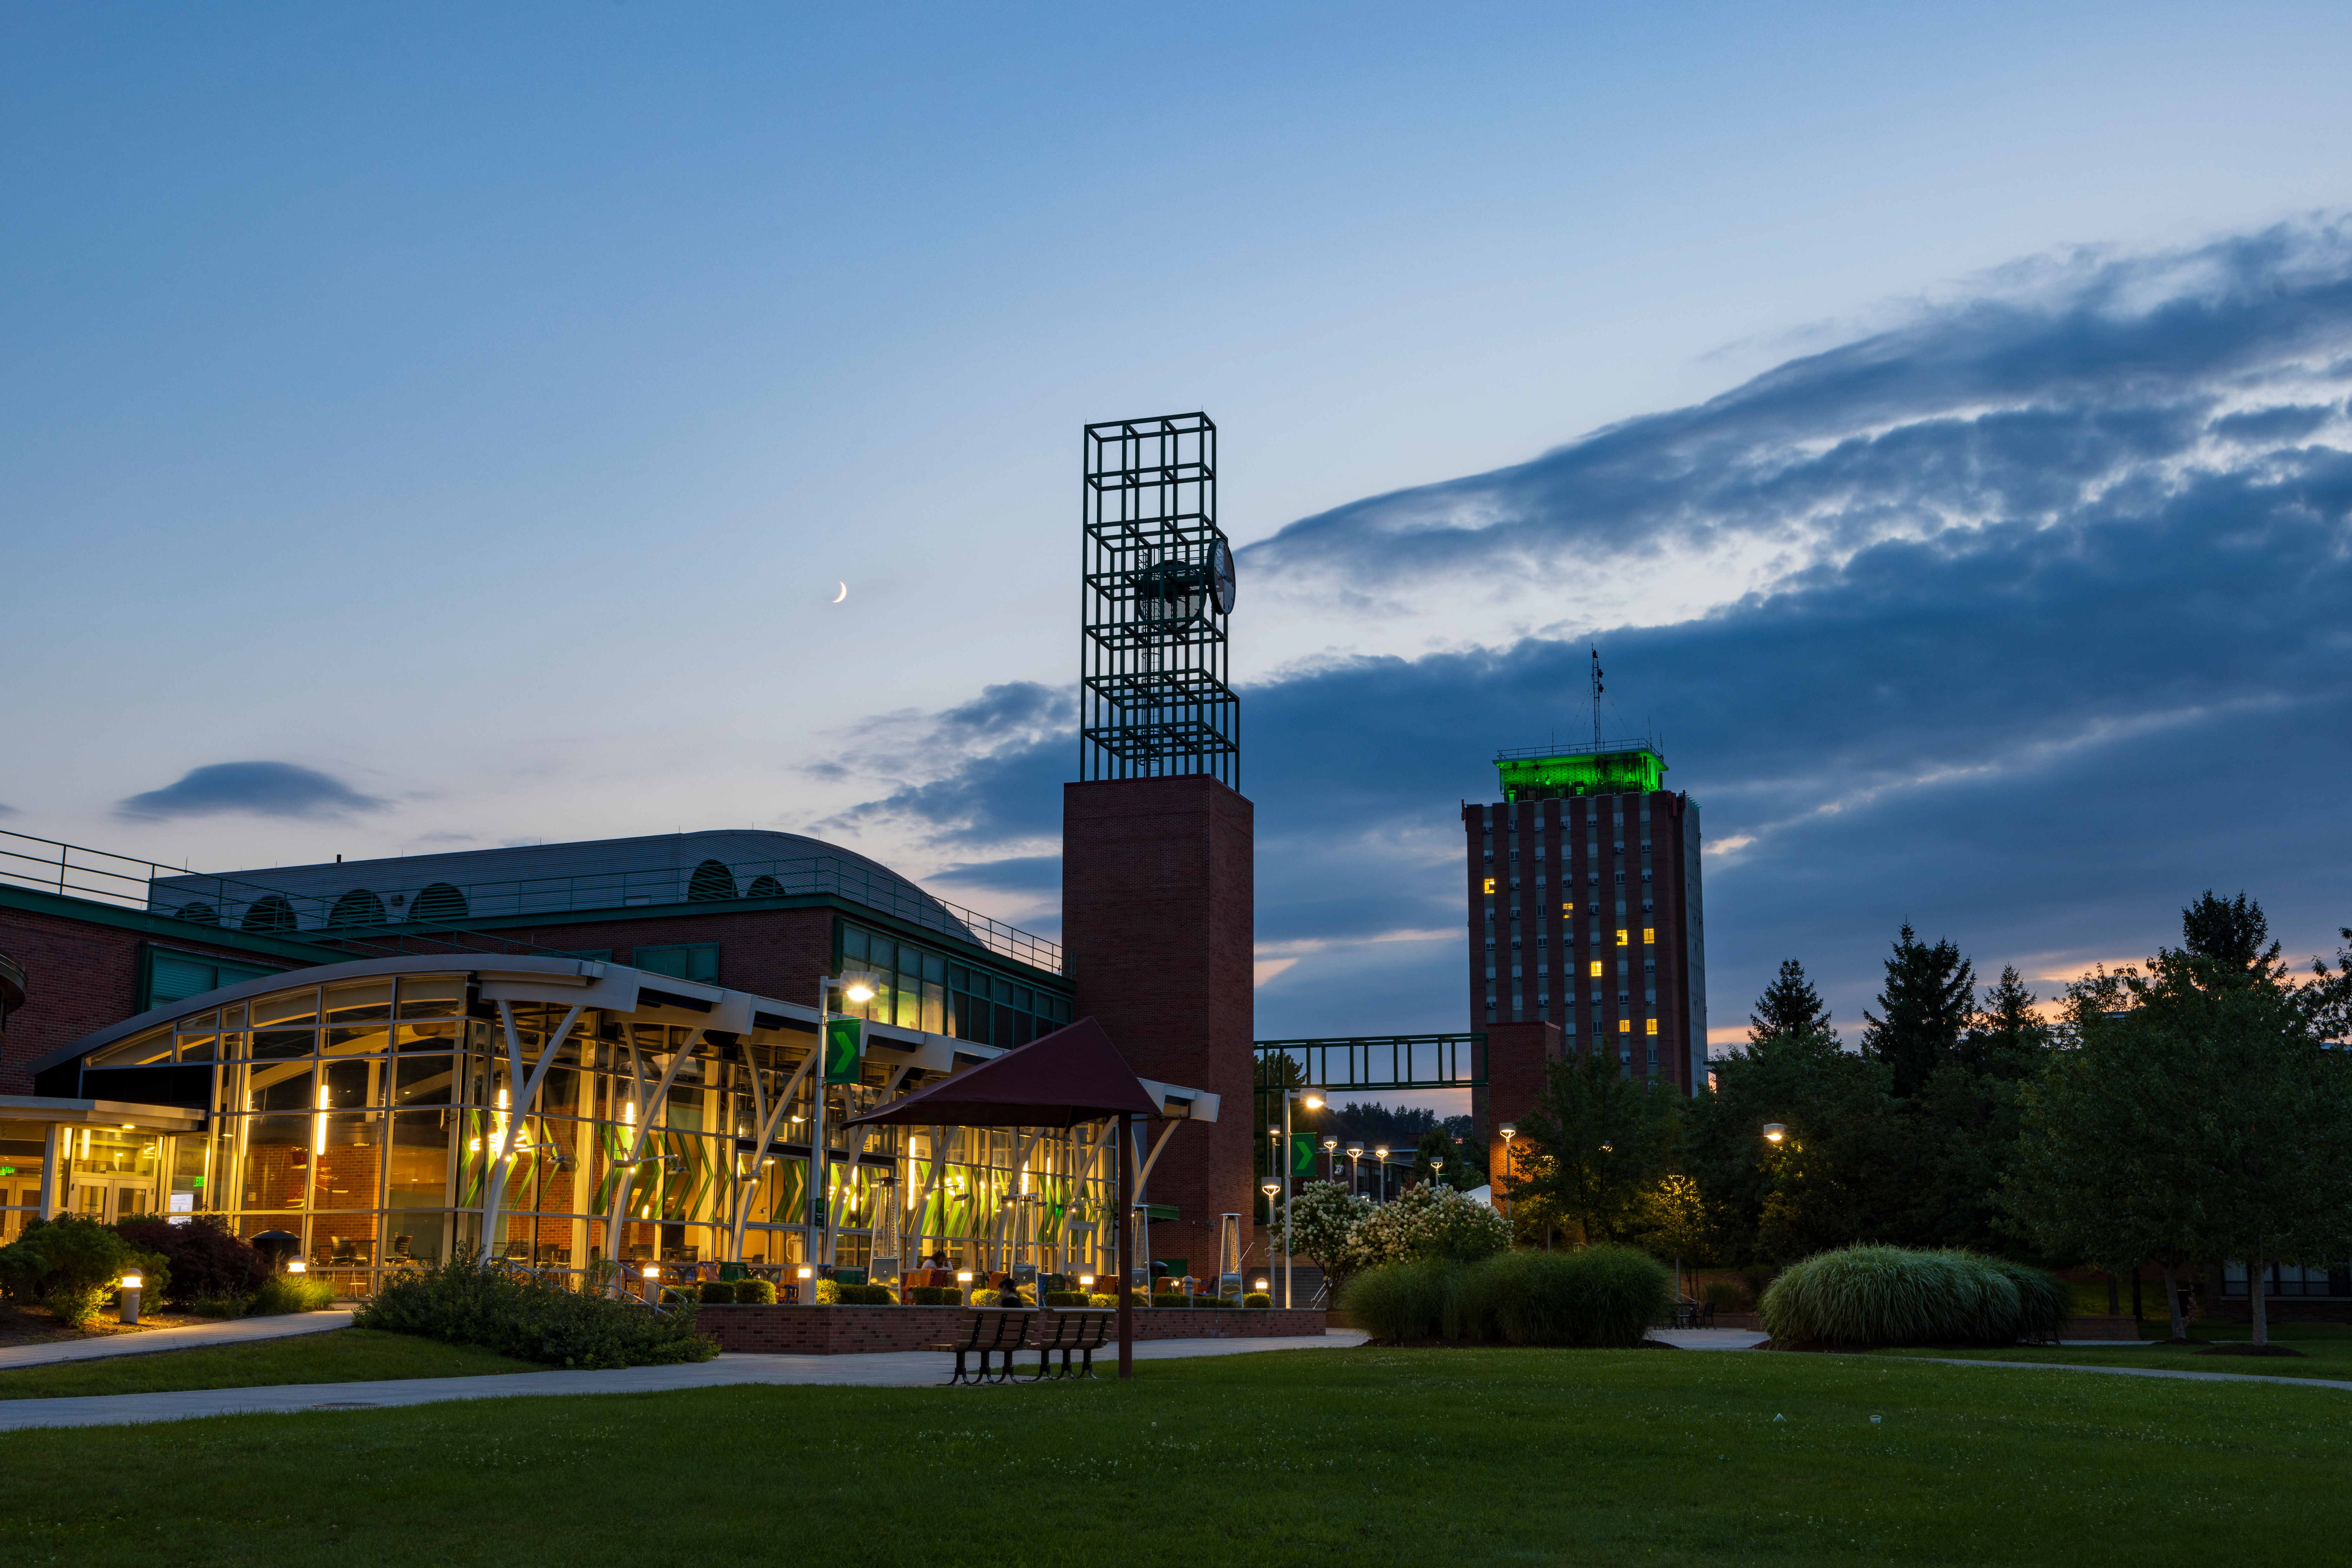
\includegraphics[width=.85\textheight]{photograph.jpg}}
    \caption{The crescent moon sets over the Clock Tower at the Union and the Glenn G. Bartle Library Tower at sunset, August 20, 2023.~\cite{BinghamtonUniversity2023Crescent}}
    \label{fig:photograph}
\end{figure}

\blindtext

\begin{figure}[t]
    \centering
    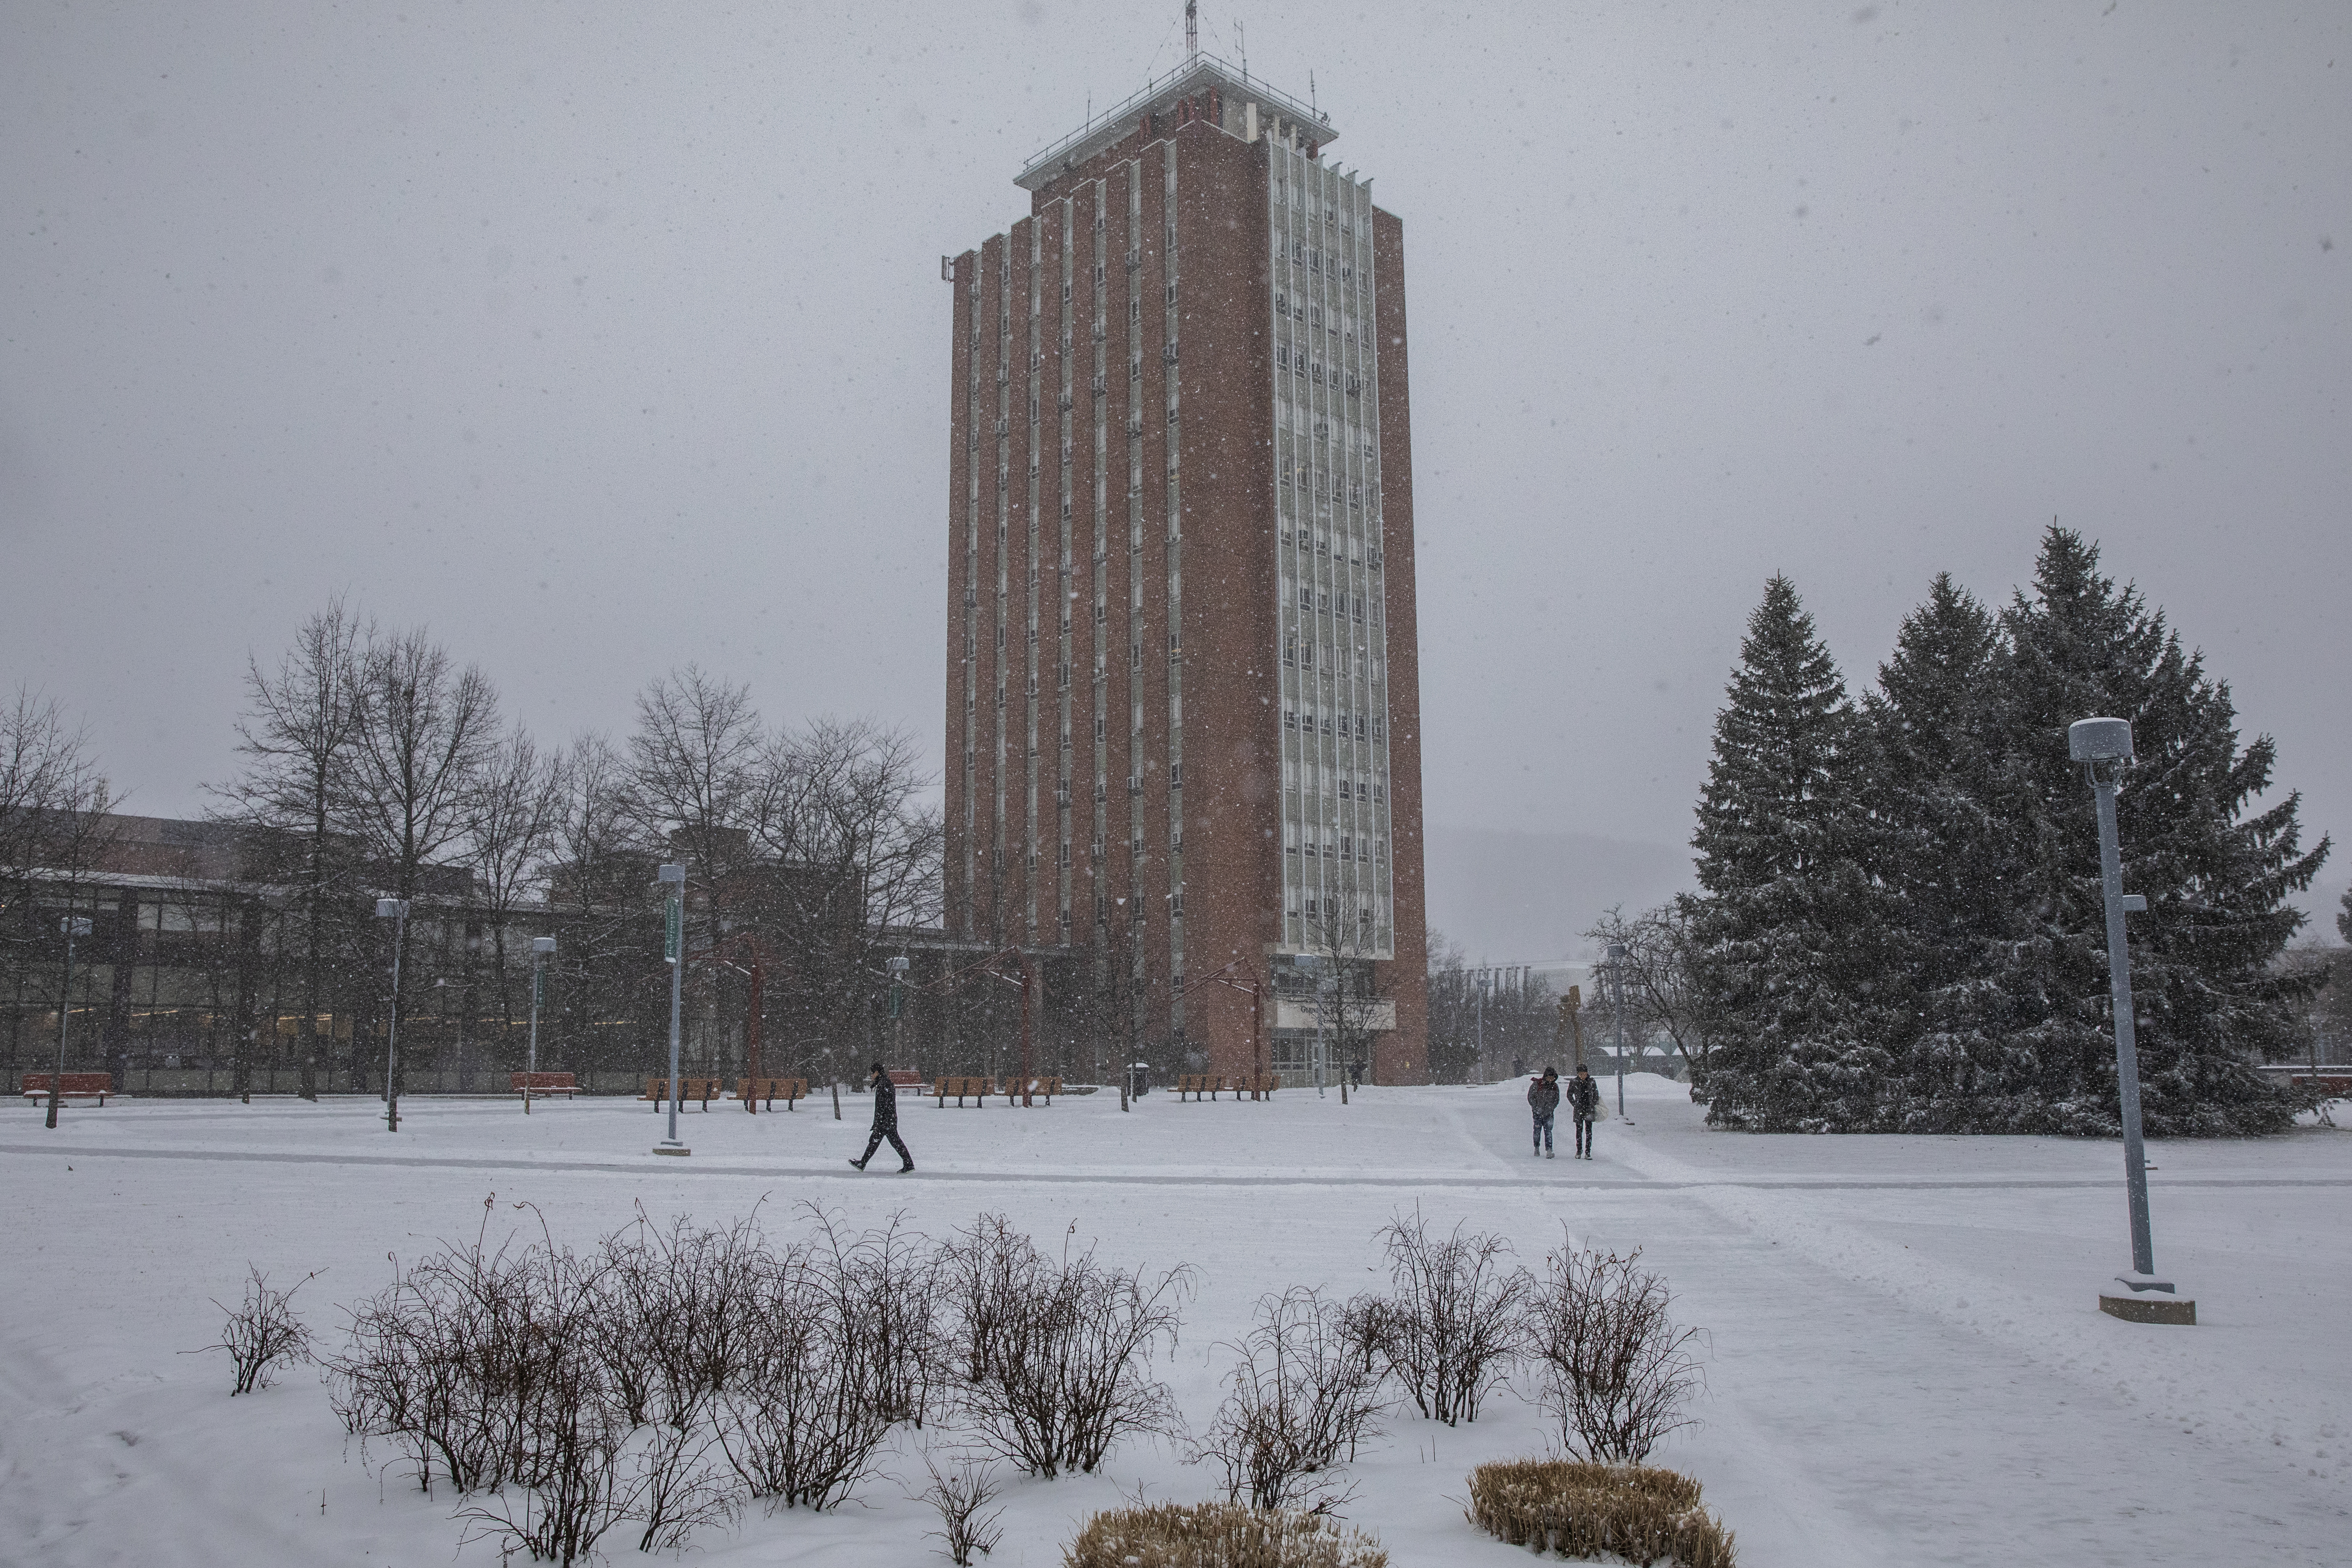
\includegraphics[scale=0.2]{figures/photograph2.jpg}
    \caption{Snowfall at Binghamton University, Tuesday, February 12, 2019. Glenn G. Bartle Library tower.~\cite{BinghamtonUniversity2023Snowfall}}
    \label{fig:photograph2}
\end{figure}

\blindtext

% Please add the following required packages to your document preamble:
% \usepackage{graphicx}
\begin{table}[p]
    \resizebox{\textwidth}{!}{%
    \begin{tabular}{p{5.5cm}|p{10cm}|l}
\hline
\textbf{Formatting Requirement} &
   &
  \textbf{Fulfilled?} \\ \hline
{\textbf{Page margins}} &
  1.5" left margin, 1" all other margins. The 1.5" left margin leaves room for the manuscript to be bound &
   \\ \hline
{\textbf{Body text of manuscript}} &
  Double-spaced. Justifying the text at the right margin is optional &
   \\ \hline
{\textbf{Font size}} &
  No smaller than 10-point and no larger than 14-point &
   \\ \hline
{\textbf{Text color}} &
  All text should be black (including URLs) &
   \\ \hline
{\textbf{New chapter}} &
  Each chapter begins at the top of a new page, with a 2" top margin &
   \\ \hline
{\textbf{Prefatory headings, chapter names, and section headings}} &
  All prefatory headings, chapter names, and section headings should be formatted consistently &
   \\ \hline
{\textbf{Footnotes or endnotes}} &
  Single-spaced, with a double space between each note &
   \\ \hline
{\textbf{Bibliographic entries, works cited, references}} &
  Single-spaced, with an extra space between entries. Style and format should otherwise follow the style guide used for the rest of the thesis/dissertation &
   \\ \hline
{\textbf{Long quotations}} &
  May be indented and single-spaced, though some style guides prefer them to be indented and double-spaced &
   \\ \hline
{\textbf{Tables and figures}} &
  Must conform to the same margins as the text. If the table or figure is placed in landscape orientation (horizontally on page), the margins and page-number location must retain a portrait (vertical) orientation, as on a regular page. Tables and figures may be in color &
   \\ \hline
{\textbf{Table and figure captions}} &
  Single spaced. Should be in the same type as the body of the text &
   \\ \hline
{\textbf{Hand lettering}} &
  Not permitted. Symbols, accent marks, and equations must be typescript &
   \\ \hline
{\textbf{Corrections in pen or pencil}} &
  Not permitted &
   \\ \hline
{\textbf{Printed manuscript}} &
  Single-sided (simplex). Do not staple. Do not hole-punch. The manuscript should be clearly readable throughout, for both electronic and printed documents. Any photocopies should be checked to make sure they are legible. If there are questions regarding print quality, you are encouraged to consult The Graduate School &
   \\ \hline
\end{tabular}%
    }
    \caption{General formatting requirements for thesis or dissertation}
    \label{tab:general-formatting}
\end{table}
    \input{chapters/blindchapter}
\end{doublespacing}

% Uncomment this line to add appendices
\appendix
\chapter{First Appendix Title}

\begin{doublespace}
    \blindtext
\end{doublespace}


\backmatter
% Uncomment this line to add endnotes section
\include{pages/notes}

\raggedright
\printbibliography[heading=bibintoc]

\end{document}
